\chapter{Background Research}
\label{chapter2}

\section{Problem Overview}
\lipsum[1-1] \cite{parikh1980adaptive}

\section{Virtual Reality}
	Virtual Reality is a technology that has been around since the early 19th century, although in a primitive form through the use of stereoscopic photos \cite{stereoscopy}. Stereoscopic photos work by using two photos that are taken of the same place but are slightly offset from each other, as can be seen in \ref{fig:stereoscope1}. This creates an illusion of depth for the person viewing the images, when viewed through a stereoscope. A stereoscope is a viewing device that only allows one eye to see one of the two images, so each eye sees a similar, yet different image, and this gives the illusion of depth. Stereoscopic vision is the same technology used in current Virtual Reality headsets although now the images are moving.\\


\begin{figure}[H]
	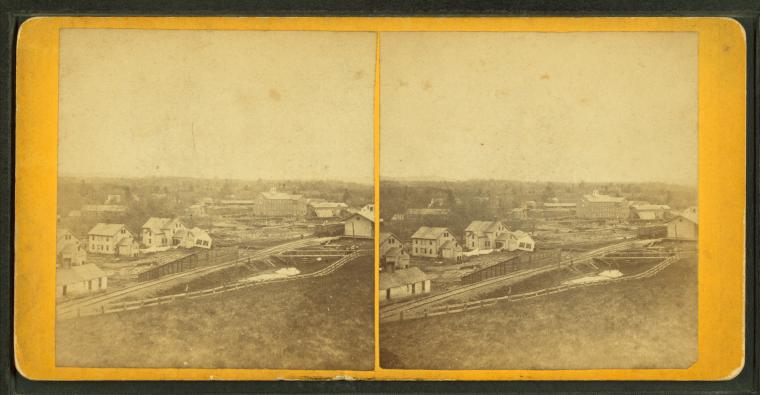
\includegraphics[width=10cm]{stereoscope}
	\centering
	\caption{Example of a stereoscopic image.}
	\label{fig:stereoscope1}
\end{figure}

	In the past couple of years the amount of consumer Virtual Reality products has increased significantly, and now there are several consumer products on the market. Examples of some are the HTC Vive, Oculus Rift, Samsung Gear VR and the Google Cardboard.

\subsection{Mobile VR}
On the market right now there are two different Mobile Virtual Reality hardware. There is the Samsung Gear VR and the Google Cardboard.

\subsubsection{Google Cardboard}
The Google Cardboard is the cheapest Virtual Reality headset out on the market right now, but it does come with the least features out of them. The cardboard viewer is a stereoscope made out of cardboard. It contains two 40mm focal lenses that are designed to give a distortion when looking through them, which is counter-acted by the distortion from the application\cite{cardboarddev}.\\
	To use the Google cardboard you would need to install the cardboard application on your compatible phone and then place your phone inside of the Google Cardboard. Once the phone is inside the Cardboard it uses the phone's inertial measurement unit to track head movement. This does have limitations however as the Google Cardboard does not track displacement if the user was to walk in any direction. \\
	The Google Cardboard still uses the technology of stereoscopic images, as can be seen in \ref{fig:cardboard1}. Although it now does it with moving images, which creates a more immersive experience. \\

\begin{figure}[H]
	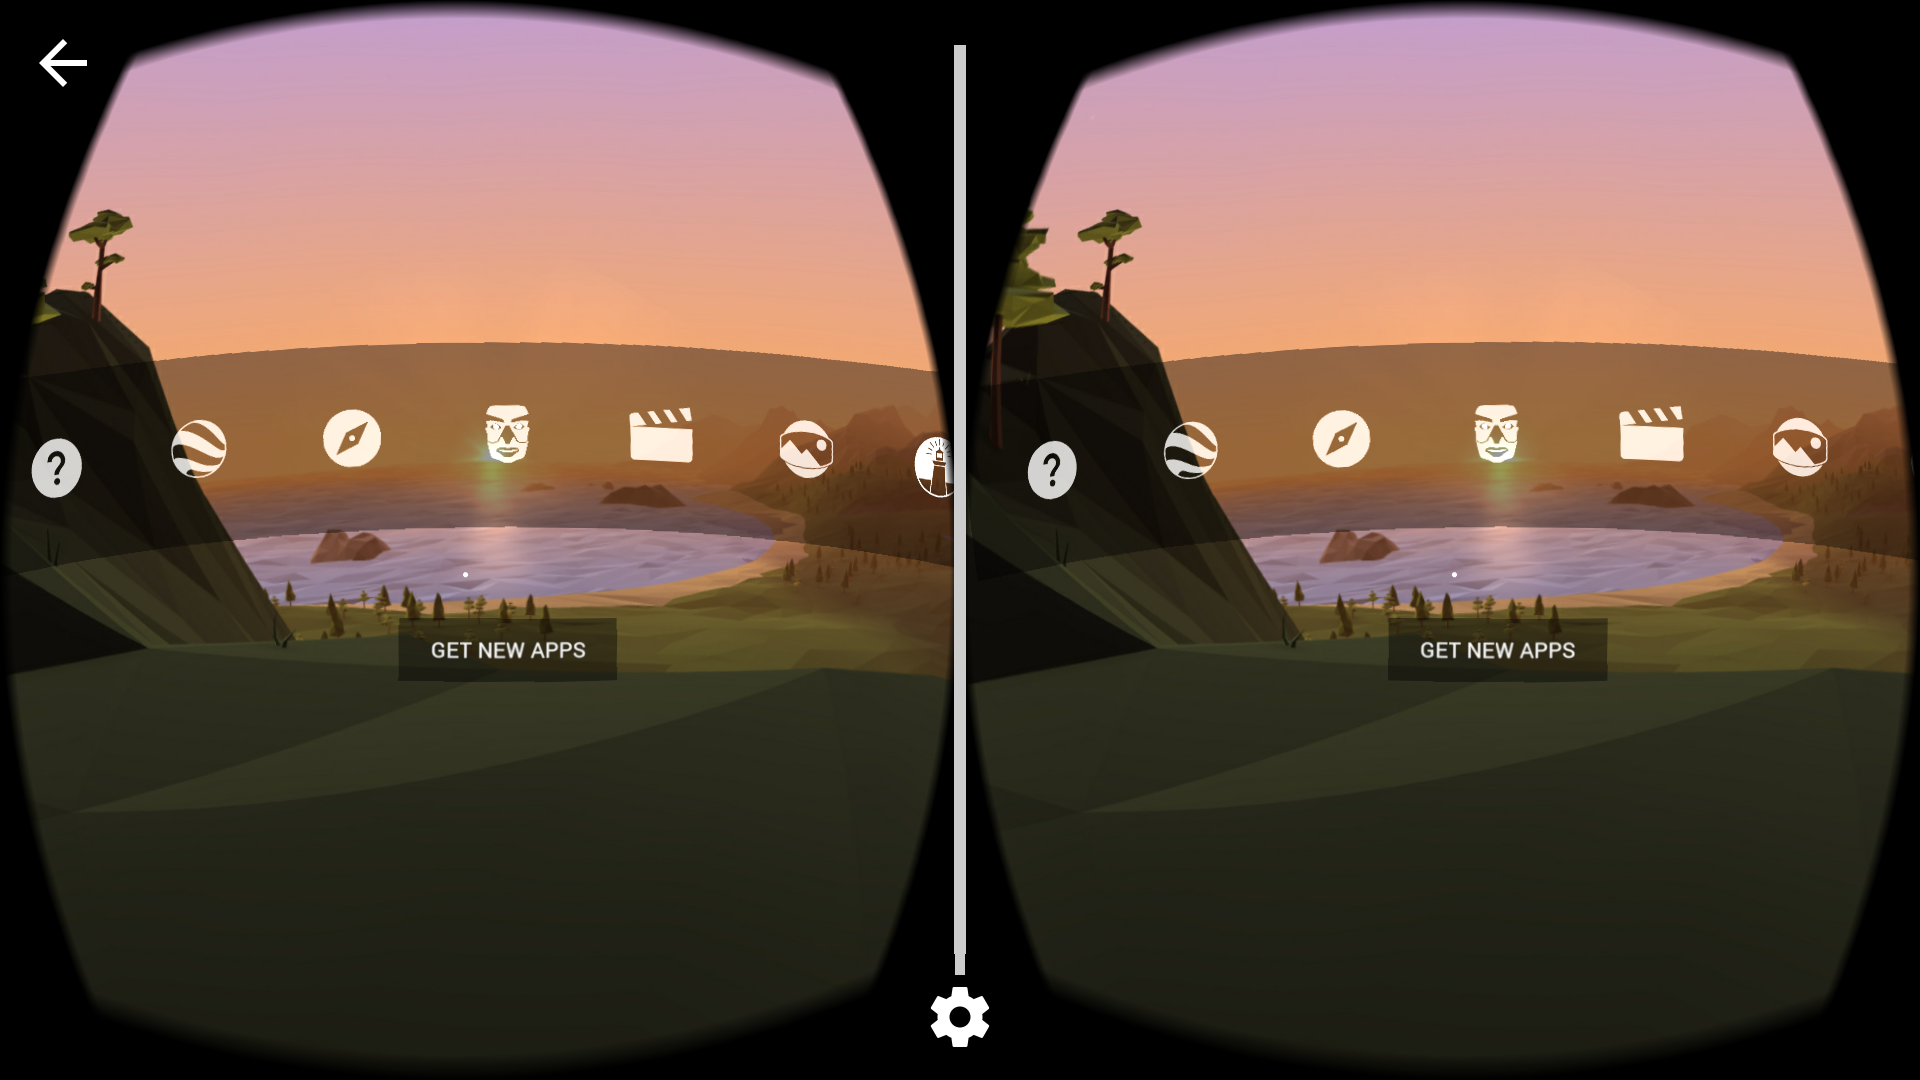
\includegraphics[width=\textwidth]{cardboardscreen}
	\centering
	\caption{Image showing the Cardboard demo application}
	\label{fig:cardboard1}
\end{figure}

	The Google Cardboard was not chosen to the virtual reality device for this project as there are many drawbacks to it, and as such it does fully demonstrate all the features present in modern technology for virtual reality. The drawbacks to the Google Cardboard are:

\begin{itemize}
	\item No displacement tracking, making it less immersive than the other options
	\item Only one input method, a button on the cardboard which acts as a screen press.
\end{itemize}

\subsubsection{Samsung Gear VR}
The other mobile Virtual Reality headset on the market is the Samsung Gear VR. The Samsung Gear VR is slightly more expensive than the Google Cardboard, and as expected with the price increase, it comes with more features compared to the Google Cardboard.\\
	The Samsung Gear VR uses the same technology as the Google Cardboard in the sense that it uses stereoscopic imaging to create the illusion of depth. This is done in the same way for both VR devices, by inserting a compatible phone into the phone holder in the headset, and then showing the stereoscopic images on the phone screen. As seen in \ref{fig:gearscreen} the Samsung gear VR uses the same stereoscopic technology as the Cardboard uses, as seen in \ref{fig:cardboard1}.\\
	The Samsung Gear VR also uses an inertial measurement unit to detect head movement, similar to the Google Cardboard. The Samsung Gear VR uses an inertial measurement unit contained in the headset, rather than using the attached phone's inertial measurement unit. The inertial measurement unit contained in the headset is more accurate, has lower latency, and is better calibrated than standard phone inertial measurement units, as it uses the same I.M.U. as the Oculus Rift. This I.M.U. is more accurate as it has a higher sample rate than internal phone I.M.U.s and therefore gives it more values to use, so that it can more accurately detect erroneous values.

\begin{figure}[H]
	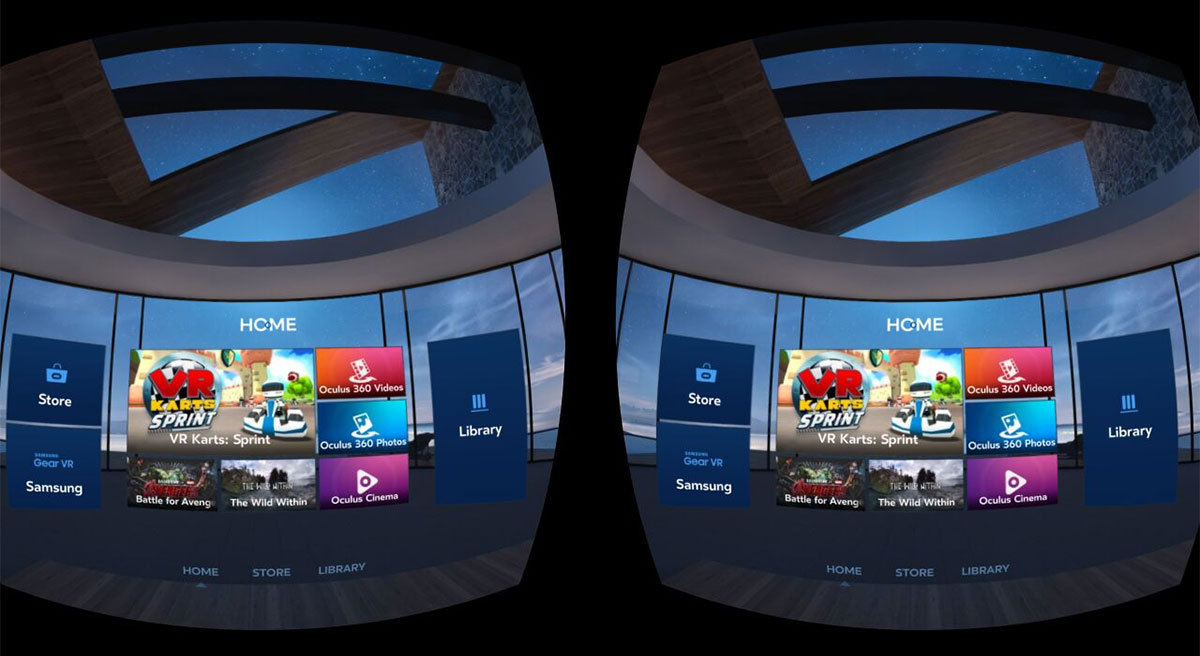
\includegraphics[width=\textwidth]{gearscreen}
	\centering
	\caption{Image showing the Samsung Gear VR menu}
	\label{fig:gearscreen}
\end{figure}

	The Samsung Gear VR has a few extra features compared to the Google Cardboard, for example when a phone is placed inside the Galaxy Gear VR it needs to be connected by a micro-usb connection, which allows the headset to have more input methods to the phone, as well as giving access to the headset's I.M.U. The extra input methods that the Gear VR has access to are:\\

\begin{itemize}
	\item A home button, which works the same as the home button on Android phones.
	\item A back button, which works the same as the back button on Android phones.
	\item A touch pad, which works by swiping to move across menus, and tapping clicks the highlighted item in a menu.
\end{itemize}

\begin{figure}[H]
	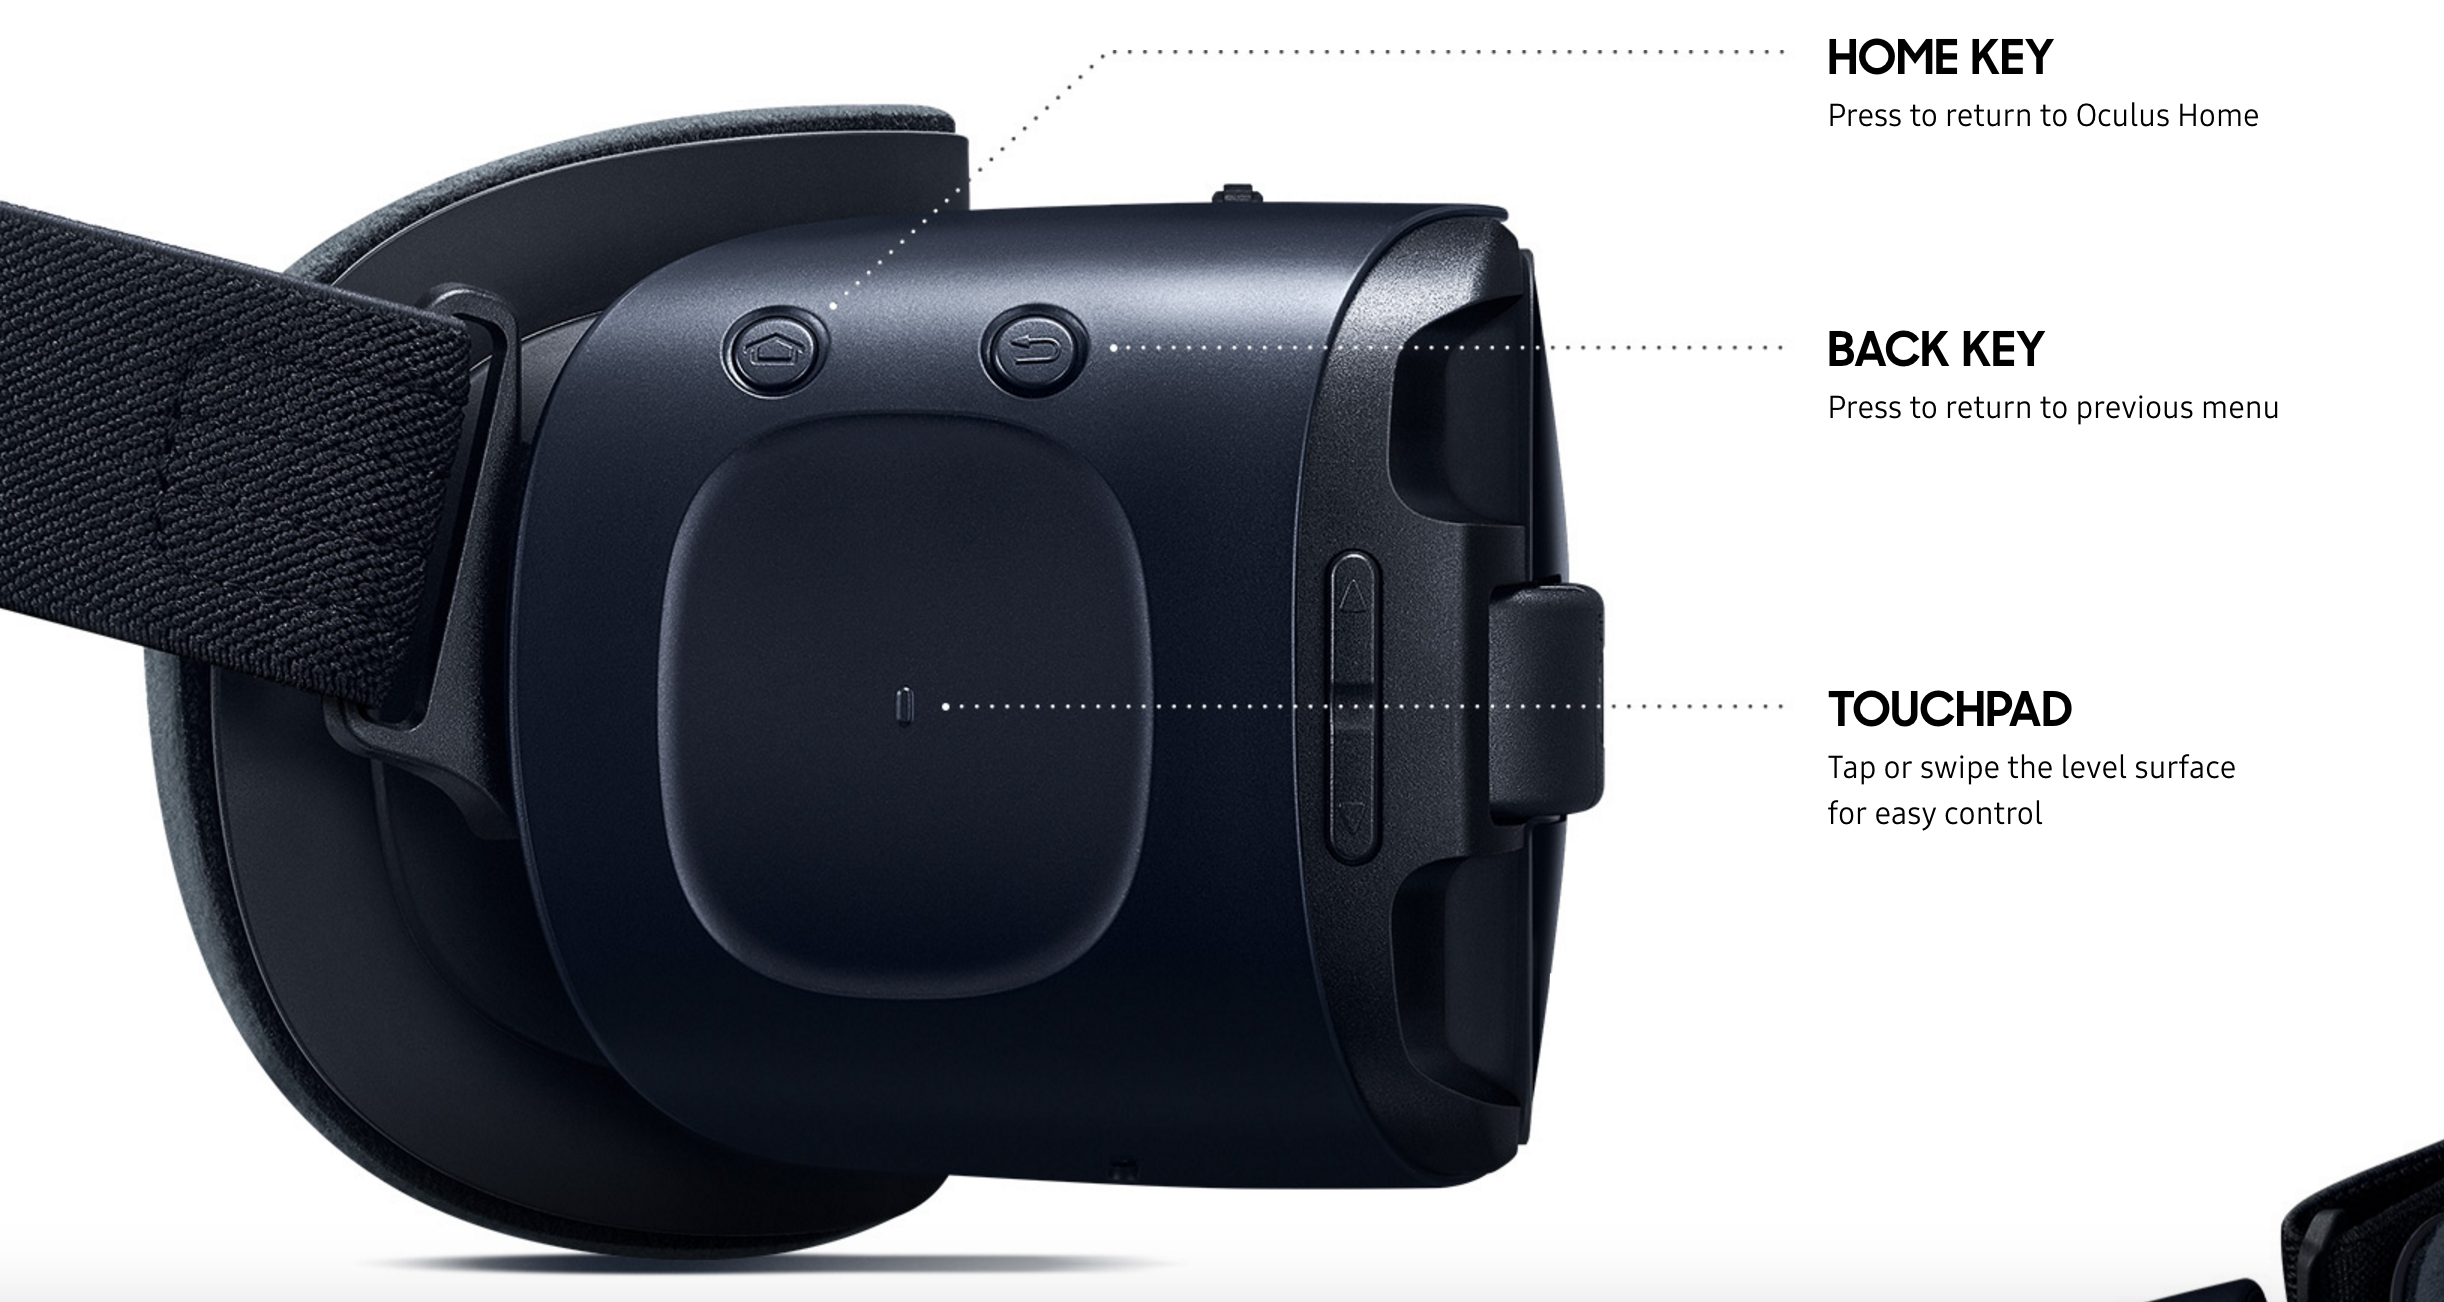
\includegraphics[width=\textwidth]{gearcontrols}
	\centering
	\caption{Image showing the hardware controls on the Samsung Gear VR}
	\label{fig:gearcontrols}
\end{figure}

	The Samsung Gear VR will not be used for this project as again it has several drawbacks, which are:

\begin{itemize}
	\item It only tracks rotational movement, not displacement, which makes it less immersive than the other options
	\item The Samsung Gear VR has very primitive control, which are only the buttons and touchpad on the side of the headset
\end{itemize}		


\subsection{Oculus Rift}
\lipsum[1-1] \cite{parikh1980adaptive}

\subsection{HTC Vive}
\lipsum[1-1] \cite{parikh1980adaptive}

\section{Gaming}
\lipsum[1-1] \cite{parikh1980adaptive}

\section{Development Environments}
\lipsum[1-1] \cite{parikh1980adaptive}

\subsection{HTC Vive}
\lipsum[1-1]

\subsection{Oculus Rift}
\lipsum[1-1]